Historii psaní dokumentů jsme si popsali v minulé kapitole, nyní je čas popsat princip, kterým dokumenty vznikají. Vznik dokumentů totiž také prochází
vývojem, ale tento vývoj přichází až v poslední době s rozvojem informačních technologí. Tvorba dokumentů by se dala rozdělit na dva různé přístupy.
Jeden má za výsledek jeden soubor, který tvoří daný dokument a druhý pouze složí dokument z určitých částí.

Než si ovšem popíše tyto dva přístupy, je nutné se podívat jak vlastně dokument vzniká. Nejdříve je nutné vytvořit návrh neboli se také používá
označení draft. Tento draft je pouze základní obrys toho co by měl výsledný dokument obsahovat. Pokud se na dokumentu podílí vícero autorů, je
tento draft kontrolován každým z nich. Z draftu se potom začne rozvíjet výsledný dokument, který se po dopsání předává ke kontrole editorům,
kde se kontroluje pravopis a stylistika. Po konečné kontrole díla autorem či autory je dílo předáno distributorovi. Celý tento postup
je znázorněn na grafu \ref{fig:linflow}

\begin{figure}[h]
    \centering
    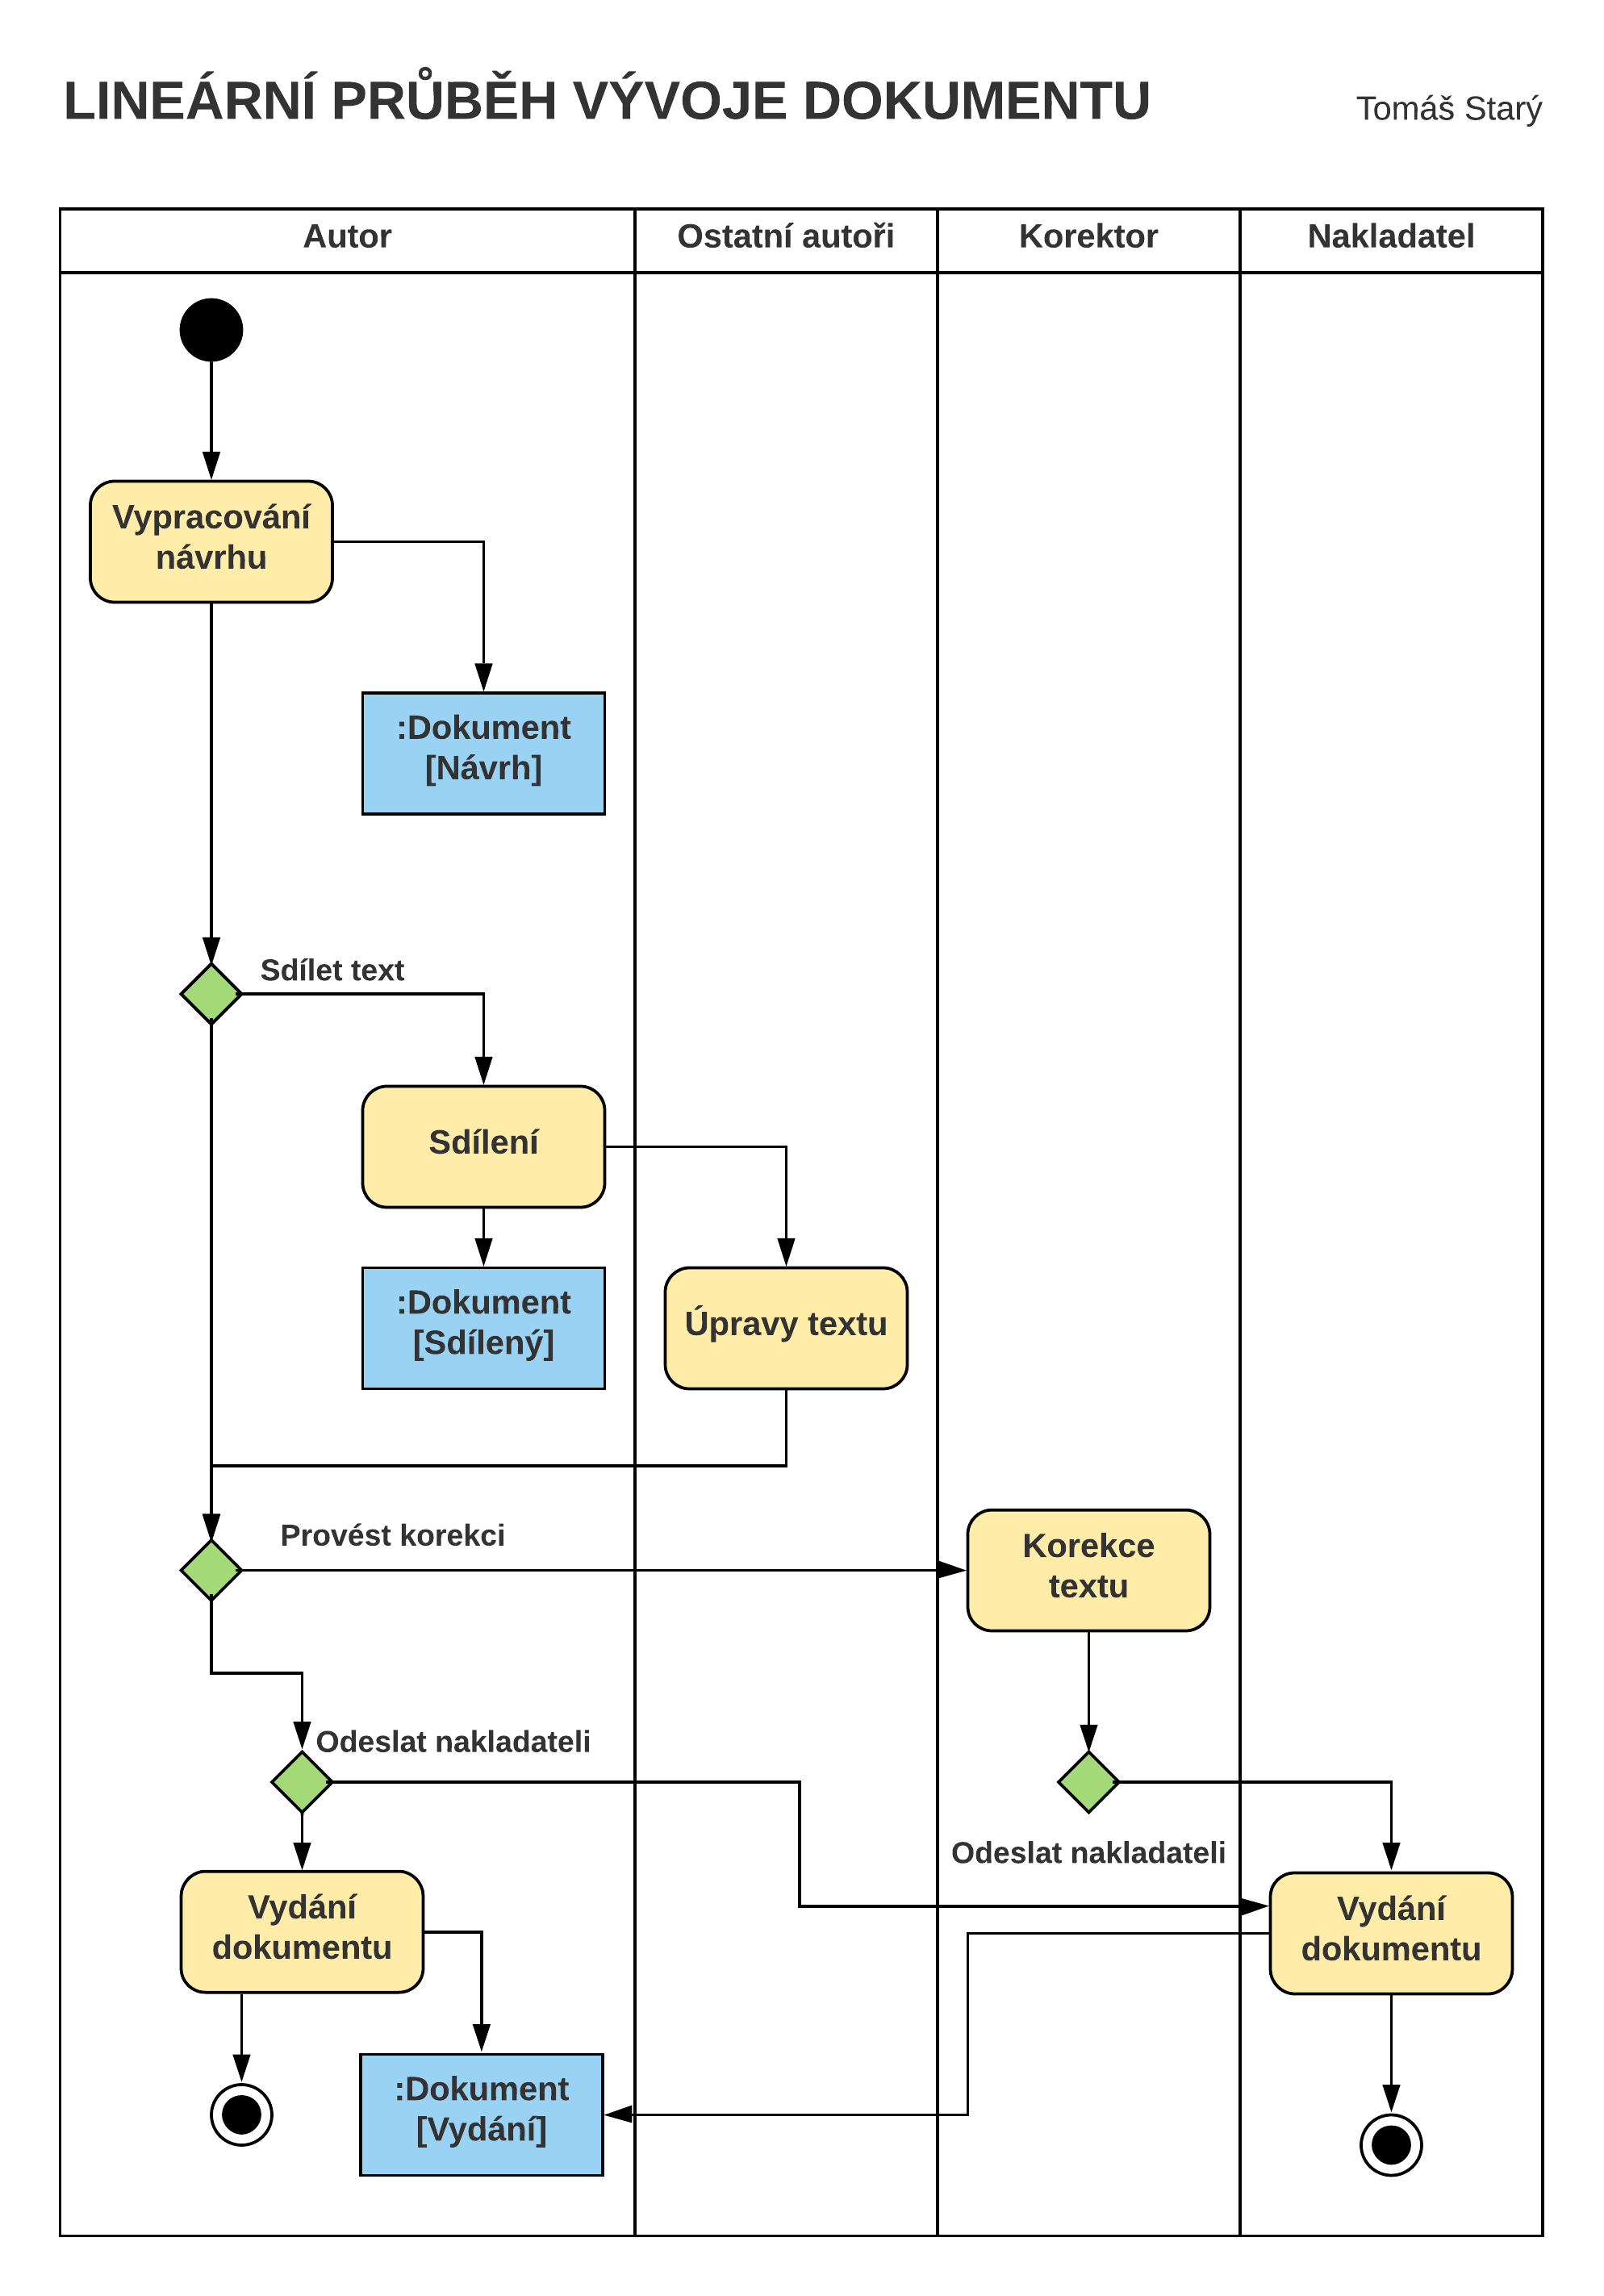
\includegraphics[width=\textwidth]{linearni_prubeh.png}
    \caption{Swimlines diagram}
    \label{fig:linflow}
\end{figure}

\section{TBA: Opak modulárního}

\subsection{Markdown}

\section{Modulární přístup}

Popis modulárního přístupu

\subsection{\LaTeX}